\documentclass{beamer}
\usetheme{Madrid}
\usecolortheme{default}
\usepackage{tikz}
\usepackage{amsmath}
\usepackage{amssymb}
\usepackage{array}

\title{Introduction to Formal Logic}
\subtitle{From Everyday Reasoning to Symbolic Systems}
\author{Brendan Shea, PhD}
\date{Intro to Logic}

\begin{document}
	
	\frame{\titlepage}
	
	\begin{frame}{From Everyday Reasoning to Formal Logic}
		\begin{itemize}
			\item We've spent the year studying how people \textbf{actually reason} in everyday life through informal logic.
			\item Today, we'll explore \textbf{formal logic}: a system that uses symbols and strict rules to analyze arguments.
			\item Think of formal logic as the mathematics of reasoning—it gives us precise tools to test whether arguments work.
			\item Just as algebra uses $x$ and $y$ instead of specific numbers, formal logic uses symbols instead of specific statements.
		\end{itemize}
		
		\begin{alertblock}{Key Insight}
			Formal logic strips away the content of arguments to focus purely on their structure.
		\end{alertblock}
	\end{frame}
	
	\begin{frame}{What Makes Logic "Formal"?}
		\begin{itemize}
			\item \textbf{Formal} means we follow exact rules, like a game with strict instructions that never change.
			\item We use \textbf{symbols} ($\wedge$, $\vee$, $\neg$, $\rightarrow$) instead of words like "and," "or," "not," and "if...then."
			\item The \textbf{validity} of an argument depends only on its form, not whether the statements are actually true.
			\item This approach eliminates ambiguity—each symbol has exactly one meaning, unlike words in natural language.
		\end{itemize}
		
		\begin{example}
			In everyday language, "or" can be inclusive (pizza or salad or both) or exclusive (boy or girl). In formal logic, $\vee$ always means inclusive or.
		\end{example}
	\end{frame}
	
	\begin{frame}{Why Study Formal Logic?}
		\begin{itemize}
			\item Formal logic is the foundation of \textbf{computer programming}—every if-then statement in code uses logical principles.
			\item It helps us spot \textbf{invalid arguments} even when they sound convincing in everyday language.
			\item Mathematics and science rely on formal logic to prove theorems and test hypotheses rigorously.
			\item Understanding formal logic makes you a more \textbf{precise thinker} and better at constructing bulletproof arguments.
		\end{itemize}
		
		\begin{block}{Three Systems We'll Explore}
			\begin{enumerate}
				\item \textbf{Categorical Logic}: Deals with categories and membership
				\item \textbf{Propositional Logic}: Connects whole statements
				\item \textbf{Predicate Logic}: Analyzes internal structure of statements
			\end{enumerate}
		\end{block}
	\end{frame}
	
	\begin{frame}{Categories and Classes: The Building Blocks}
		\begin{itemize}
			\item \textbf{Categorical logic} studies relationships between groups or classes of things.
			\item A \textbf{category} is any collection we can clearly define: wizards, muggles, Hogwarts students, magical creatures.
			\item We examine how categories relate through \textbf{inclusion} (all wizards are magical), \textbf{exclusion} (no muggles are wizards), and \textbf{overlap} (some students are wizards).
			\item Every statement in categorical logic makes a claim about the relationship between two categories.
		\end{itemize}
		
		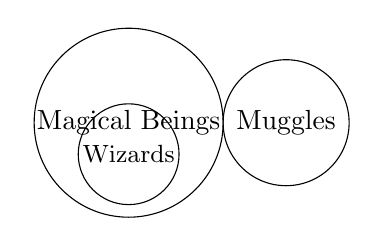
\begin{tikzpicture}[scale=0.8]
			\draw (0,0) circle (1.5cm) node {Magical Beings};
			\draw (0,-0.5) circle (0.8cm) node[font=\small] {Wizards};
			\draw (2.5,0) circle (1cm) node {Muggles};
		\end{tikzpicture}
	\end{frame}
	
	\begin{frame}{The Four Standard Forms (A, E, I, O)}
		\begin{itemize}
			\item \textbf{A-form (Universal Affirmative)}: "All S are P" — All Gryffindors are brave.
			\item \textbf{E-form (Universal Negative)}: "No S are P" — No Death Eaters are kind.  
			\item \textbf{I-form (Particular Affirmative)}: "Some S are P" — Some wizards are Animagi.
			\item \textbf{O-form (Particular Negative)}: "Some S are not P" — Some students are not Quidditch players.
		\end{itemize}
		
		\begin{block}{Key Terms}
			\begin{tabular}{ll}
				\textbf{Universal} & Refers to every member of a category \\
				\textbf{Particular} & Refers to at least one member \\
				\textbf{Affirmative} & States inclusion or membership \\
				\textbf{Negative} & States exclusion or non-membership
			\end{tabular}
		\end{block}
	\end{frame}
	
	\begin{frame}{Venn Diagrams: Visualizing Relationships}
		\begin{itemize}
			\item \textbf{Venn diagrams} use overlapping circles to show relationships between categories visually.
			\item Shading indicates \textbf{empty regions} (no members exist there), while X marks show \textbf{existing members}.
			\item Each of our four forms (A, E, I, O) has a unique Venn diagram pattern.
			\item These diagrams help us test whether arguments are valid by checking if conclusions must follow from premises.
		\end{itemize}
		
\begin{example}
\begin{columns}
	\column{0.5\textwidth}
	\scriptsize
	“All Elves are Immortal” (A-form)
	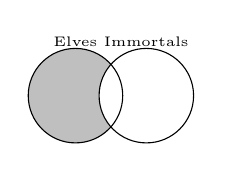
\begin{tikzpicture}[scale=0.6]
		% Draw the two sets
	
		% Shade entire Elves circle
		\fill[gray,opacity=0.5] (0,0) circle (1cm);
		% Erase the overlap by painting Immortals circle white
		\fill[white] (1.5,0) circle (1cm);
		\draw (0,0) circle (1cm) node[above=.5cm] {\tiny Elves};
		\draw (1.5,0) circle (1cm) node[above=.5cm] {\tiny Immortals};
	\end{tikzpicture}
	\column{0.5\textwidth}
	The left circle (Elves) outside the overlap is shaded, showing all Elves must be in the Immortal category.
\end{columns}
\end{example}
\end{frame}
	
	\begin{frame}{Sample Argument: All Dogs Are Mammals}
		\begin{itemize}
			\item Let's analyze a classic \textbf{syllogism} (an argument with two premises and a conclusion).
			\item \textbf{Premise 1}: All hobbits are Middle-earth dwellers.
			\item \textbf{Premise 2}: All Middle-earth dwellers are fictional characters.
			\item \textbf{Conclusion}: Therefore, Therefore, all hobbits are fictional characters.
		\end{itemize}
		
		\begin{alertblock}{Valid Argument Structure}
			This follows the pattern called \textbf{Barbara}: All A are B, All B are C, therefore All A are C. The conclusion must be true if both premises are true.
		\end{alertblock}
	\end{frame}
	
	\begin{frame}{Practice: Translating Everyday Claims}
		\begin{itemize}
			\item Natural language is often ambiguous, so we must \textbf{standardize} statements into A, E, I, or O forms.
			\item "Jedi never use the dark side" becomes "\textbf{No Jedi are dark side users}" (E-form).
			\item "Not all heroes wear capes" becomes "\textbf{Some heroes are not cape-wearers}" (O-form).
			\item Watch for hidden quantifiers: "Dragons breathe fire" usually means "\textbf{All dragons} breathe fire" (A-form).
		\end{itemize}
		
		\begin{block}{Translation Tips}
			\begin{tabular}{ll}
				"Only X are Y" & = "All Y are X" (reversed!) \\
				"X are always Y" & = "All X are Y" \\
				"There are X that Y" & = "Some X are Y" \\
				"Not every X is Y" & = "Some X are not Y"
			\end{tabular}
		\end{block}
	\end{frame}
	
	\begin{frame}{The Square of Opposition}
		\begin{itemize}
			\item The \textbf{Square of Opposition} shows logical relationships between the four categorical forms.
			\item \textbf{Contradictories} (A-O, E-I) cannot both be true or both be false—exactly one must be true.
			\item \textbf{Contraries} (A-E) cannot both be true, but both can be false.
			\item \textbf{Subcontraries} (I-O) cannot both be false, but both can be true.
		\end{itemize}
		
		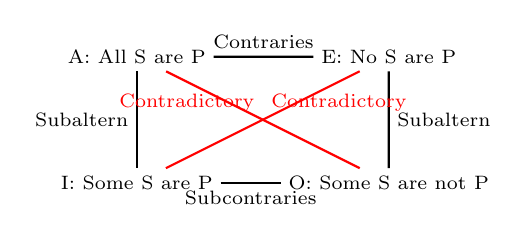
\begin{tikzpicture}[scale=0.8]
			\scriptsize
			% Square
			\node (A) at (0,2) {A: All S are P};
			\node (E) at (4,2) {E: No S are P};
			\node (I) at (0,0) {I: Some S are P};
			\node (O) at (4,0) {O: Some S are not P};
			
			% Lines
			\draw[thick] (A) -- (E) node[midway,above] {Contraries};
			\draw[thick] (I) -- (O) node[midway,below] {Subcontraries};
			\draw[thick] (A) -- (I) node[midway,left] {Subaltern};
			\draw[thick] (E) -- (O) node[midway,right] {Subaltern};
			\draw[thick,red] (A) -- (O) node[midway,above right] {Contradictory};
			\draw[thick,red] (E) -- (I) node[midway,above left] {Contradictory};
		\end{tikzpicture}
	\end{frame}
	

	
	\begin{frame}{From Categories to Propositions}
		\begin{itemize}
			\item While categorical logic focuses on relationships between groups, \textbf{propositional logic} works with complete statements.
			\item A \textbf{proposition} is any statement that can be true or false: "Harry defeated Voldemort," "It's raining," "2+2=4."
			\item Instead of analyzing internal structure, propositional logic examines how we \textbf{connect} statements using logical operators.
			\item This system is more flexible—we can analyze any argument made of statements, not just those about categories.
		\end{itemize}
		
		\begin{alertblock}{Key Shift}
			Categorical logic asks "What's inside statements?" while propositional logic asks "How do statements connect?"
		\end{alertblock}
	\end{frame}
		\begin{frame}{Basic Connectives: AND, OR, NOT}
		\begin{itemize}
			\item \textbf{Conjunction} ($\wedge$, AND): "Hermione is smart $\wedge$ Hermione is brave" — both parts must be true.
			\item \textbf{Disjunction} ($\vee$, OR): "Ron plays chess $\vee$ Ron plays Quidditch" — at least one part must be true.
			\item \textbf{Negation} ($\neg$, NOT): "$\neg$ Voldemort has a nose" — reverses the truth value.
			\item These \textbf{logical connectives} are the building blocks for creating complex propositions from simple ones.
		\end{itemize}
		
		\begin{block}{Formal Notation}
			\begin{tabular}{lll}
				\textbf{Connective} & \textbf{Symbol} & \textbf{Example} \\
				\hline
				AND & $\wedge$ & $p \wedge q$ \\
				OR & $\vee$ & $p \vee q$ \\
				NOT & $\neg$ & $\neg p$ \\
				IF...THEN & $\rightarrow$ & $p \rightarrow q$ \\
				IF AND ONLY IF & $\leftrightarrow$ & $p \leftrightarrow q$
			\end{tabular}
		\end{block}
	\end{frame}
	
	\begin{frame}{Truth Tables: The Foundation}
		\begin{itemize}
			\item A \textbf{truth table} shows all possible combinations of truth values for propositions and their results.
			\item Each row represents one possible scenario, and we calculate the truth value of complex expressions.
			\item Truth tables give us a mechanical way to determine when compound statements are true or false.
			\item They're like multiplication tables for logic—once you know them, you can solve any problem!
		\end{itemize}
		
		\begin{example}
			Truth table for $p \wedge q$ (Frodo has the ring AND Sam helps him):
			\begin{center}
				\begin{tabular}{|c|c|c|}
					\hline
					$p$ & $q$ & $p \wedge q$ \\
					\hline
					T & T & T \\
					T & F & F \\
					F & T & F \\
					F & F & F \\
					\hline
				\end{tabular}
			\end{center}
			Only true when BOTH parts are true!
		\end{example}
	\end{frame}
	
	\begin{frame}{Sample Argument: If-Then Reasoning}
		\begin{itemize}
			\item The \textbf{conditional} ($\rightarrow$) represents "if...then" statements: "If you're a wizard, then you can do magic."
			\item $p \rightarrow q$ is only false when $p$ is true but $q$ is false (you're a wizard but can't do magic).
			\item This captures cause-and-effect, rules, and logical consequences in a precise way.
			\item Be careful: "If $p$ then $q$" does NOT mean "$q$ only if $p$"—muggles might do magic too!
		\end{itemize}
		
		\begin{alertblock}{Common Confusion}
			"If you eat the poison apple, then you fall asleep" ($p \rightarrow q$)\\
			This does NOT mean: "You fall asleep only if you eat the poison apple"\\
			Sleeping pills could also make you fall asleep!
		\end{alertblock}
	\end{frame}
	
	\begin{frame}{Complex Propositions: Building Bigger Claims}
		\begin{itemize}
			\item We can combine multiple connectives to build \textbf{complex propositions} that capture sophisticated ideas.
			\item Use parentheses to show order of operations: $(p \wedge q) \rightarrow r$ differs from $p \wedge (q \rightarrow r)$.
			\item Each added connective doubles the rows in our truth table—complexity grows exponentially!
			\item Real arguments often involve many connected statements working together.
		\end{itemize}
		
		\begin{example}
			"If Gandalf arrives and the weather is good, then we'll defeat Sauron or retreat to safety"
			\begin{center}
				Let $g$ = Gandalf arrives, $w$ = weather is good,\\
				$d$ = defeat Sauron, $r$ = retreat to safety
				
				Formula: $(g \wedge w) \rightarrow (d \vee r)$
			\end{center}
			This has $2^4 = 16$ rows in its truth table!
		\end{example}
	\end{frame}
	
	\begin{frame}{Valid vs. Invalid Categorical Arguments}
		\begin{itemize}
			\item A \textbf{valid} argument guarantees that if the premises are true, the conclusion must be true.
			\item An \textbf{invalid} argument can have true premises but a false conclusion—the logic doesn't work.
			\item We test validity by checking whether the conclusion's Venn diagram is already contained in the premises' diagrams.
			\item Remember: validity is about structure, not truth—an argument can be valid with false premises!
		\end{itemize}
		
		\begin{example}
			\textbf{Invalid Argument}:
			\begin{enumerate}
				\item All Time Lords have two hearts. (True in Doctor Who universe)
				\item The Doctor has two hearts. (True)
				\item Therefore, the Doctor is a Time Lord. (Doesn't follow!)
			\end{enumerate}
			This commits the fallacy of \textbf{affirming the consequent}—other beings might also have two hearts.
		\end{example}
	\end{frame}
	
	\begin{frame}{Practice: Translating Natural Language}
		\begin{itemize}
			\item Natural language hides logical structure, so we must identify the \textbf{atomic propositions} and \textbf{connectives}.
			\item "You can't apparate in Hogwarts" becomes $\neg p$ where $p$ = "You can apparate in Hogwarts."
			\item "Either die a hero or live long enough to become the villain" becomes $h \vee v$ (inclusive or!).
			\item "I'll help if and only if you're truly sorry" becomes $h \leftrightarrow s$ (biconditional).
		\end{itemize}
		
		\begin{block}{Translation Strategy}
			\begin{enumerate}
				\item Identify each distinct claim that can be true/false
				\item Assign a letter to each atomic proposition
				\item Find the logical connectives (and, or, not, if...then)
				\item Build the formula using proper symbols
			\end{enumerate}
		\end{block}
	\end{frame}
	
	\begin{frame}{Common Valid Forms: Modus Ponens}
		\begin{itemize}
			\item \textbf{Modus Ponens} ("method of affirming") is a fundamental valid argument form.
			\item Structure: If $p$ then $q$; $p$ is true; therefore $q$ is true.
			\item This pattern appears everywhere in mathematical proofs, computer programs, and daily reasoning.
			\item It's so basic that denying it would make logical reasoning impossible!
		\end{itemize}
		
		\begin{example}
			\textbf{Modus Ponens in Action}:
			\begin{enumerate}
				\item If you speak Parseltongue, then you can open the Chamber. $(p \rightarrow q)$
				\item Harry speaks Parseltongue. $(p)$
				\item Therefore, Harry can open the Chamber. $(q)$
			\end{enumerate}
			
			Truth table confirms: whenever both premises are true, conclusion must be true.
		\end{example}
	\end{frame}
	
	\begin{frame}{Common Invalid Forms: Affirming the Consequent}
		\begin{itemize}
			\item \textbf{Affirming the Consequent} looks similar to Modus Ponens but is invalid.
			\item Structure: If $p$ then $q$; $q$ is true; therefore $p$ is true. (WRONG!)
			\item This fallacy assumes there's only one way for $q$ to be true, ignoring other possibilities.
			\item It's tempting because it seems to work backwards from effects to causes.
		\end{itemize}
		
		\begin{alertblock}{Invalid Reasoning}
			\begin{enumerate}
				\item If you're a Death Eater, then you have the Dark Mark. $(p \rightarrow q)$
				\item Karkaroff has the Dark Mark. $(q)$
				\item Therefore, Karkaroff is a Death Eater. $(p)$ — INVALID!
			\end{enumerate}
			Why invalid? Former Death Eaters keep their marks!
		\end{alertblock}
	\end{frame}
	
	\begin{frame}{Using Truth Tables to Test Validity}
		\begin{itemize}
			\item To test validity, we build a truth table with columns for all premises and the conclusion.
			\item An argument is \textbf{valid} if every row where ALL premises are true also has a true conclusion.
			\item If even one row has true premises but false conclusion, the argument is \textbf{invalid}.
			\item This method is foolproof but can be tedious for complex arguments with many propositions.
		\end{itemize}
		
		\begin{example}
			Testing: $p \rightarrow q, \neg q \therefore \neg p$ (Modus Tollens)
			\begin{center}
				\begin{tabular}{|c|c|c|c|c|c|}
					\hline
					$p$ & $q$ & $p \rightarrow q$ & $\neg q$ & $\neg p$ & Valid? \\
					\hline
					T & T & T & F & F & — \\
					T & F & F & T & F & — \\
					F & T & T & F & T & — \\
					F & F & T & T & T & \checkmark \\
					\hline
				\end{tabular}
			\end{center}
			Only row 4 has both premises true, and conclusion is true there!
		\end{example}
	\end{frame}
	
	\begin{frame}{The Limits of Propositional Logic}
		\begin{itemize}
			\item Propositional logic treats "Socrates is mortal" as a single, indivisible unit $p$.
			\item It can't express the connection between "Socrates is mortal" and "Plato is mortal"—they're just unrelated $p$ and $q$.
			\item We lose important patterns: "All X are Y" requires a different proposition for each X!
			\item Mathematical statements like "For every number $n$, there exists $n+1$" are impossible to express properly.
		\end{itemize}
		
		\begin{alertblock}{The Problem}
			In propositional logic, these require different symbols:
			\begin{itemize}
				\item $p$: Harry is a wizard
				\item $q$: Ron is a wizard  
				\item $r$: Hermione is a wizard
			\end{itemize}
			We can't capture that they all share the property "is a wizard"!
		\end{alertblock}
	\end{frame}
	
	\begin{frame}{Why We Need More Power}
		\begin{itemize}
			\item Real reasoning often involves \textbf{generalizations} about entire groups or categories.
			\item We need to express \textbf{relationships} and \textbf{properties} that apply to many individuals.
			\item Mathematical proofs require statements about "all numbers" or "there exists a solution."
			\item \textbf{Predicate logic} provides tools to look inside propositions and work with their structure.
		\end{itemize}
		
		\begin{block}{What Predicate Logic Adds}
			\begin{enumerate}
				\item \textbf{Predicates}: Properties or relations (like "is red" or "is taller than")
				\item \textbf{Variables}: Stand-ins for individuals (like $x$, $y$ in algebra)
				\item \textbf{Quantifiers}: "For all" ($\forall$) and "There exists" ($\exists$)
				\item \textbf{Domain}: The universe of things we're talking about
			\end{enumerate}
		\end{block}
	\end{frame}
	
	\begin{frame}{Introducing Predicates and Subjects}
		\begin{itemize}
			\item A \textbf{predicate} is a property or relation that can be true or false of individuals.
			\item \textbf{Subjects} are the specific individuals we're talking about (Harry, the number 7, this pencil).
			\item We write $P(a)$ to mean "individual $a$ has property $P$"—like $Wizard(Harry)$ for "Harry is a wizard."
			\item Relations between multiple subjects use multiple places: $Loves(Romeo, Juliet)$ means "Romeo loves Juliet."
		\end{itemize}
		
		\begin{example}
			Breaking down "Gandalf is wise and helps Frodo":
			\begin{itemize}
				\item Predicates: $Wise(x)$ = "$x$ is wise", $Helps(x,y)$ = "$x$ helps $y$"
				\item Subjects: $g$ = Gandalf, $f$ = Frodo
				\item Formula: $Wise(g) \wedge Helps(g,f)$
			\end{itemize}
		\end{example}
	\end{frame}
	
	\begin{frame}{From "Socrates is mortal" to Mx}
		\begin{itemize}
			\item The classic statement "Socrates is mortal" becomes $Mortal(socrates)$ or $Ms$ for short.
			\item We can now express patterns: $Mortal(socrates)$, $Mortal(plato)$, $Mortal(aristotle)$ all use the same predicate!
			\item \textbf{Predicate symbols} (usually capital letters) represent properties: $M$, $P$, $Q$.
			\item \textbf{Constant symbols} (usually lowercase) represent specific individuals: $a$, $b$, $c$.
		\end{itemize}
		
		\begin{block}{Building Our Vocabulary}
			\begin{tabular}{ll}
				$Jedi(x)$ & $x$ is a Jedi \\
				$Teaches(x,y)$ & $x$ teaches $y$ \\
				$Stronger(x,y)$ & $x$ is stronger than $y$ \\
				$yoda$, $luke$, $obiwan$ & Individual constants
			\end{tabular}
		\end{block}
	\end{frame}
	
	\begin{frame}{Variables: The x in Predicate Logic}
		\begin{itemize}
			\item \textbf{Variables} (usually $x$, $y$, $z$) are placeholders that can represent any individual in our domain.
			\item Just like in algebra where $x$ can be any number, in logic $x$ can be any person, object, or entity.
			\item $P(x)$ is not a complete statement—it's a \textbf{formula with a free variable} that becomes true/false when we specify $x$.
			\item Variables let us express general patterns before we commit to specific individuals.
		\end{itemize}
		
		\begin{example}
			The formula $Wizard(x) \wedge Teaches(x, harry)$ means "$x$ is a wizard and $x$ teaches Harry"
			\begin{itemize}
				\item If $x$ = Dumbledore: TRUE (he's a wizard who teaches Harry)
				\item If $x$ = Snape: TRUE (also a wizard teacher)  
				\item If $x$ = Hagrid: FALSE (teaches Harry but isn't a wizard)
			\end{itemize}
		\end{example}
	\end{frame}
	
	\begin{frame}{The Universal Quantifier: $\forall$ (For All)}
		\begin{itemize}
			\item The \textbf{universal quantifier} $\forall$ means "for all" or "for every" individual in our domain.
			\item $\forall x P(x)$ reads as "For all $x$, $P(x)$ is true" or "Everything has property $P$."
			\item This captures universal claims like "All ravens are black" as $\forall x (Raven(x) \rightarrow Black(x))$.
			\item The quantifier \textbf{binds} the variable—$\forall x P(x)$ is a complete statement that's either true or false.
		\end{itemize}
		
		\begin{alertblock}{Important Pattern}
			Universal statements usually use implication:
			\begin{itemize}
				\item "All wizards can do magic" = $\forall x (Wizard(x) \rightarrow CanDoMagic(x))$
				\item NOT: $\forall x (Wizard(x) \wedge CanDoMagic(x))$ — this says everything is a wizard!
			\end{itemize}
		\end{alertblock}
	\end{frame}
	
	\begin{frame}{The Existential Quantifier: $\exists$ (There Exists)}
		\begin{itemize}
			\item The \textbf{existential quantifier} $\exists$ means "there exists at least one" or "for some."
			\item $\exists x P(x)$ reads as "There exists an $x$ such that $P(x)$ is true" or "Something has property $P$."
			\item This captures claims like "Some dragons are friendly" as $\exists x (Dragon(x) \wedge Friendly(x))$.
			\item To make an existential statement true, we only need to find ONE example that works.
		\end{itemize}
		
		\begin{block}{Contrast with Universal}
			\begin{tabular}{ll}
				\textbf{Universal} & \textbf{Existential} \\
				\hline
				$\forall x (Elf(x) \rightarrow Immortal(x))$ & $\exists x (Elf(x) \wedge Mortal(x))$ \\
				"All elves are immortal" & "Some elf is mortal" \\
				Uses implication ($\rightarrow$) & Uses conjunction ($\wedge$) \\
				False if ONE counterexample & True if ONE example exists
			\end{tabular}
		\end{block}
	\end{frame}
	
	\begin{frame}{Sample Translation: "All Students Study"}
		\begin{itemize}
			\item English: "All students study" seems simple but hides logical complexity.
			\item First identify predicates: $Student(x)$ = "$x$ is a student", $Studies(x)$ = "$x$ studies."
			\item The logical form is: $\forall x (Student(x) \rightarrow Studies(x))$.
			\item Read carefully: "For any individual $x$, IF $x$ is a student, THEN $x$ studies."
		\end{itemize}
		
		\begin{example}
			Let's check if our translation works correctly:
			\begin{itemize}
				\item Hermione (student who studies): $Student(h) \rightarrow Studies(h)$ is $T \rightarrow T = T$ \checkmark
				\item Dobby (non-student): $Student(d) \rightarrow Studies(d)$ is $F \rightarrow ? = T$ \checkmark
				\item Ron (student who doesn't study): $Student(r) \rightarrow Studies(r)$ is $T \rightarrow F = F$ $\times$
			\end{itemize}
			The formula is false only when we find a student who doesn't study!
		\end{example}
	\end{frame}
	
	\begin{frame}{Sample Translation: "Some Books Are Interesting"}
		\begin{itemize}
			\item English: "Some books are interesting" claims at least one interesting book exists.
			\item Predicates: $Book(x)$ = "$x$ is a book", $Interesting(x)$ = "$x$ is interesting."
			\item The logical form is: $\exists x (Book(x) \wedge Interesting(x))$.
			\item Read as: "There exists an $x$ such that $x$ is a book AND $x$ is interesting."
		\end{itemize}
		
		\begin{alertblock}{Why Conjunction, Not Implication?}
			Compare these formulas:
			\begin{itemize}
				\item $\exists x (Book(x) \wedge Interesting(x))$ — "Some book is interesting" \checkmark
				\item $\exists x (Book(x) \rightarrow Interesting(x))$ — "There's something such that IF it's a book THEN it's interesting"
			\end{itemize}
			The second is true whenever ANY non-book exists (like a pencil)!
		\end{alertblock}
	\end{frame}
	
	\begin{frame}{Combining Quantifiers and Connectives}
		\begin{itemize}
			\item We can mix quantifiers with all our logical connectives for complex statements.
			\item "No Death Eaters are kind" becomes $\forall x (DeathEater(x) \rightarrow \neg Kind(x))$.
			\item "Only wizards can see Thestrals" becomes $\forall x (SeesThestrals(x) \rightarrow Wizard(x))$.
			\item Parentheses matter: $\forall x (P(x) \wedge Q(x))$ differs from $\forall x P(x) \wedge \forall x Q(x)$!
		\end{itemize}
		
		\begin{example}
			"Not all that glitters is gold" translation:
			\begin{enumerate}
				\item First attempt: $\neg \forall x (Glitters(x) \rightarrow Gold(x))$ 
				\item Equivalent: $\exists x (Glitters(x) \wedge \neg Gold(x))$
				\item Read as: "Something glitters but isn't gold"
			\end{enumerate}
			Both forms say the same thing using logical equivalences!
		\end{example}
	\end{frame}
	
	\begin{frame}{Multiple Quantifiers: Order Matters!}
		\begin{itemize}
			\item When using multiple quantifiers, their \textbf{order changes the meaning} dramatically.
			\item $\forall x \exists y Loves(x,y)$ means "Everyone loves someone" (each person might love someone different).
			\item $\exists y \forall x Loves(x,y)$ means "There's someone whom everyone loves" (one universally loved person).
			\item Read quantifiers from left to right, with each one setting up context for the next.
		\end{itemize}
		
		\begin{block}{The Difference Illustrated}
			\begin{tabular}{ll}
				$\forall x \exists y Teaches(x,y)$ & Every teacher has (at least) one student \\
				$\exists y \forall x Teaches(x,y)$ & One super-student is taught by everyone \\
				$\exists x \forall y Teaches(x,y)$ & One super-teacher teaches everyone \\
				$\forall y \exists x Teaches(x,y)$ & Every student has (at least) one teacher
			\end{tabular}
		\end{block}
	\end{frame}
	
	\begin{frame}{Practice: "Everyone Loves Someone"}
		\begin{itemize}
			\item This classic example shows why quantifier order is crucial for correct translation.
			\item Ambiguous English: "Everyone loves someone" has two possible meanings!
			\item \textbf{Reading 1}: Each person loves at least one person (maybe different for each).
			\item \textbf{Reading 2}: There's one special person whom everyone loves.
		\end{itemize}
		
		\begin{example}
			The two translations:
			\begin{enumerate}
				\item $\forall x \exists y Loves(x,y)$ — "For each $x$, there exists a $y$ that $x$ loves"
				\begin{itemize}
					\item Harry loves Ginny, Ron loves Hermione, Snape loves Lily...
				\end{itemize}
				\item $\exists y \forall x Loves(x,y)$ — "There exists a $y$ such that every $x$ loves $y$"
				\begin{itemize}
					\item Everyone loves Dumbledore (or pizza, or baby Yoda...)
				\end{itemize}
			\end{enumerate}
			English is ambiguous; predicate logic is precise!
		\end{example}
	\end{frame}
	
	\begin{frame}{Common Translation Pitfalls}
		\begin{itemize}
			\item \textbf{Pitfall 1}: Using $\wedge$ instead of $\rightarrow$ with universal quantifiers.
			\item \textbf{Pitfall 2}: Using $\rightarrow$ instead of $\wedge$ with existential quantifiers.
			\item \textbf{Pitfall 3}: Forgetting that "only" reverses the direction of implication.
			\item \textbf{Pitfall 4}: Misplacing negations—$\neg \forall x$ is very different from $\forall x \neg$!
		\end{itemize}
		
		\begin{alertblock}{Common Mistakes}
			\scriptsize
			\begin{tabular}{ll}
				\textbf{Wrong} & \textbf{Right} \\
				\hline
				"All cats meow": $\forall x (Cat(x) \wedge Meows(x))$ & $\forall x (Cat(x) \rightarrow Meows(x))$ \\
				"Some cats meow": $\exists x (Cat(x) \rightarrow Meows(x))$ & $\exists x (Cat(x) \wedge Meows(x))$ \\
				"Only cats meow": $\forall x (Cat(x) \rightarrow Meows(x))$ & $\forall x (Meows(x) \rightarrow Cat(x))$ \\
				"Not all cats meow": $\forall x \neg (Cat(x) \rightarrow Meows(x))$ & $\neg \forall x (Cat(x) \rightarrow Meows(x))$
			\end{tabular}
		\end{alertblock}
	\end{frame}
	
	\begin{frame}{The Domain of Discourse}
		\begin{itemize}
			\item The \textbf{domain of discourse} is the set of all individuals our variables can represent.
			\item Different domains can make the same formula true or false—context matters!
			\item Common domains: all people, all numbers, all living things, all objects in Middle-earth.
			\item Sometimes we restrict domains to simplify formulas: "All are brave" vs. "All hobbits are brave."
		\end{itemize}
		
		\begin{example}
			Consider $\forall x Magical(x)$ ("Everything is magical")
			\begin{itemize}
				\item Domain = \{Harry, Hermione, Dumbledore\}: TRUE \checkmark
				\item Domain = \{Harry, Hermione, Uncle Vernon\}: FALSE $\times$
				\item Domain = All characters in Harry Potter: FALSE $\times$
			\end{itemize}
			The same formula, different truth values based on domain!
		\end{example}
	\end{frame}
	
	\begin{frame}{Sample Argument: Socrates Revisited}
		\begin{itemize}
			\item Now we can properly express the classic Socrates syllogism in predicate logic.
			\item \textbf{Premise 1}: All humans are mortal — $\forall x (Human(x) \rightarrow Mortal(x))$
			\item \textbf{Premise 2}: Socrates is human — $Human(socrates)$  
			\item \textbf{Conclusion}: Socrates is mortal — $Mortal(socrates)$
		\end{itemize}
		
		\begin{block}{Why This Works}
			\begin{enumerate}
				\item From Premise 1, we know: $Human(socrates) \rightarrow Mortal(socrates)$
				\item From Premise 2, we know: $Human(socrates)$ is true
				\item By Modus Ponens: If $p \rightarrow q$ and $p$, then $q$
				\item Therefore: $Mortal(socrates)$ must be true!
			\end{enumerate}
			This is called \textbf{Universal Instantiation} followed by Modus Ponens.
		\end{block}
	\end{frame}
	
	\begin{frame}{From English to Symbols: Step by Step}
		\begin{itemize}
			\item \textbf{Step 1}: Identify the domain (what are we talking about?).
			\item \textbf{Step 2}: List needed predicates and assign letters (keep a dictionary!).
			\item \textbf{Step 3}: Identify logical structure (universal/existential, and/or/not, if/then).
			\item \textbf{Step 4}: Build the formula piece by piece, checking each part makes sense.
		\end{itemize}
		
		\begin{example}
			Translating: "Every wizard has a wand that chooses them"
			\begin{enumerate}
				\item Domain: All people and objects in the wizarding world
				\item Predicates: $Wizard(x)$, $Wand(y)$, $Chooses(y,x)$
				\item Structure: Universal (every wizard) + Existential (has a wand)
				\item Formula: $\forall x (Wizard(x) \rightarrow \exists y (Wand(y) \wedge Chooses(y,x)))$
			\end{enumerate}
		\end{example}
	\end{frame}
	
	\begin{frame}{Practice: "No Reptiles Are Warm-Blooded"}
		\begin{itemize}
			\item This negative universal statement requires careful translation to avoid errors.
			\item Predicates: $Reptile(x)$ = "$x$ is a reptile", $WarmBlooded(x)$ = "$x$ is warm-blooded"
			\item The correct translation: $\forall x (Reptile(x) \rightarrow \neg WarmBlooded(x))$
			\item Alternative equivalent form: $\neg \exists x (Reptile(x) \wedge WarmBlooded(x))$
		\end{itemize}
		
		\begin{block}{Understanding the Forms}
			\begin{tabular}{ll}
				$\forall x (Reptile(x) \rightarrow \neg WarmBlooded(x))$ & "All reptiles are not warm-blooded" \\
				$\neg \exists x (Reptile(x) \wedge WarmBlooded(x))$ & "No warm-blooded reptile exists" \\
			\end{tabular}
			Both say the same thing: you can't find a reptile that's warm-blooded!
		\end{block}
	\end{frame}
	
	\begin{frame}{Nested Quantifiers: "Every Student Has a Favorite Teacher"}
		\begin{itemize}
			\item Complex statements often involve relationships between multiple quantified variables.
			\item Predicates: $Student(x)$, $Teacher(y)$, $Favorite(x,y)$ = "$y$ is $x$'s favorite teacher"
			\item Translation: $\forall x (Student(x) \rightarrow \exists y (Teacher(y) \wedge Favorite(x,y)))$
			\item Read: "For every $x$, if $x$ is a student, then there exists a $y$ such that $y$ is a teacher and $y$ is $x$'s favorite."
		\end{itemize}
		
		\begin{example}
			Breaking down the formula structure:
			\begin{center}
				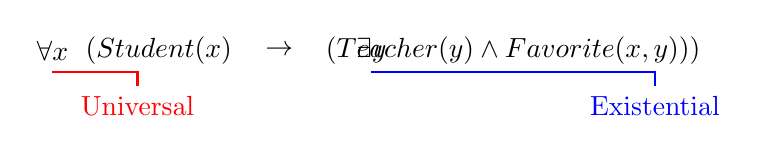
\begin{tikzpicture}[scale=0.9]
					\node at (0,0) {$\forall x$};
					\node at (1.5,0) {$(Student(x)$};
					\node at (3.2,0) {$\rightarrow$};
					\node at (4.5,0) {$\exists y$};
					\node at (6.5,0) {$(Teacher(y) \wedge Favorite(x,y)))$};
					\draw[red,thick] (0,-0.3) -- (1.2,-0.3) -- (1.2,-0.5) node[below] {Universal};
					\draw[blue,thick] (4.5,-0.3) -- (8.5,-0.3) -- (8.5,-0.5) node[below] {Existential};
				\end{tikzpicture}
			\end{center}
		\end{example}
	\end{frame}
	
	\begin{frame}{Testing Validity in Predicate Logic}
		\begin{itemize}
			\item Testing validity in predicate logic is more complex than using truth tables.
			\item We can use \textbf{natural deduction} rules like Universal Instantiation and Existential Generalization.
			\item Another method uses \textbf{semantic interpretations}: find a domain and interpretation where premises are true but conclusion is false.
			\item For simple arguments, we can still check validity by applying logical rules systematically.
		\end{itemize}
		
		\begin{alertblock}{Validity Test Example}
			\scriptsize
			Test: "All elves are immortal. Legolas is an elf. Therefore, someone is immortal."
			\begin{enumerate}
				\item $\forall x (Elf(x) \rightarrow Immortal(x))$ [Premise 1]
				\item $Elf(legolas)$ [Premise 2]
				\item $Elf(legolas) \rightarrow Immortal(legolas)$ [Universal Instantiation on 1]
				\item $Immortal(legolas)$ [Modus Ponens on 2,3]
				\item $\exists x Immortal(x)$ [Existential Generalization on 4] \checkmark
			\end{enumerate}
		\end{alertblock}
	\end{frame}
	
	\begin{frame}{Mathematical Statements in Predicate Logic}
		\begin{itemize}
			\item Predicate logic is the language of mathematics—every theorem can be expressed using quantifiers.
			\item "Every positive number has a square root": $\forall x (Positive(x) \rightarrow \exists y (y^2 = x))$
			\item "There exists a largest prime": $\exists x (Prime(x) \wedge \forall y (Prime(y) \rightarrow y \leq x))$
			\item Mathematical proofs are essentially chains of valid predicate logic arguments!
		\end{itemize}
		
		\begin{example}
			The statement "Between any two different real numbers, there's another real number":
			\begin{center}
				$\forall x \forall y ((Real(x) \wedge Real(y) \wedge x \neq y) \rightarrow$\\
				$\exists z (Real(z) \wedge ((x < z \wedge z < y) \vee (y < z \wedge z < x))))$
			\end{center}
			This captures the density property of real numbers!
		\end{example}
	\end{frame}
	
	\begin{frame}{Scientific Claims as Formal Arguments}
		\begin{itemize}
			\item Scientific hypotheses and laws can be expressed precisely using predicate logic.
			\item "All metals conduct electricity": $\forall x (Metal(x) \rightarrow ConductsElectricity(x))$
			\item "Some mutations are beneficial": $\exists x (Mutation(x) \wedge Beneficial(x))$
			\item The scientific method tests these logical claims against empirical evidence.
		\end{itemize}
		
		\begin{block}{Scientific Reasoning Pattern}
			\begin{enumerate}
				\item Hypothesis: $\forall x (P(x) \rightarrow Q(x))$ (All P's have property Q)
				\item Test case: Find some $a$ where $P(a)$ is true
				\item Prediction: $Q(a)$ should be true
				\item If $\neg Q(a)$: Hypothesis is falsified!
			\end{enumerate}
			This is the logical structure behind Karl Popper's falsificationism.
		\end{block}
	\end{frame}
	
	\begin{frame}{Computer Science and Logic}
		\begin{itemize}
			\item Every computer program is built on formal logic—if statements, loops, and boolean operations.
			\item Database queries use predicate logic: SQL's WHERE clause is essentially a logical formula!
			\item \textbf{Program verification} proves code correctness using predicate logic assertions.
			\item Artificial Intelligence systems use logic for knowledge representation and reasoning.
		\end{itemize}
		
	\end{frame}
	
	\begin{frame}{Common Logical Errors in Everyday Life}
		\begin{itemize}
			\item \textbf{Hasty Generalization}: Concluding $\forall x P(x)$ from just a few examples.
			\item \textbf{Denying the Antecedent}: From $p \rightarrow q$ and $\neg p$, concluding $\neg q$ (invalid!).
			\item \textbf{Quantifier Confusion}: Mixing up "all" and "some" in complex statements.
			\item \textbf{Correlation/Causation}: Observing $\forall x (P(x) \leftrightarrow Q(x))$ but claiming $P$ causes $Q$.
		\end{itemize}
		
		\begin{alertblock}{Real-World Example}
			"Everyone who recovered took the medicine, so the medicine cured them."
			\begin{itemize}
				\item Observation: $\forall x (Recovered(x) \rightarrow TookMedicine(x))$
				\item Invalid conclusion: $\forall x (TookMedicine(x) \rightarrow Recovered(x))$
				\item This reverses the implication! (Affirming the consequent)
			\end{itemize}
		\end{alertblock}
	\end{frame}
	
	\begin{frame}{The Power and Limits of Formal Logic}
		\begin{itemize}
			\item \textbf{Power}: Formal logic gives us certainty—valid arguments guarantee true conclusions from true premises.
			\item \textbf{Power}: It's universal—the same rules work for math, science, philosophy, and daily reasoning.
			\item \textbf{Limit}: Logic alone can't tell us which premises are actually true in the real world.
			\item \textbf{Limit}: Many important human concepts (beauty, justice, meaning) resist complete formalization.
		\end{itemize}
		
		\begin{block}{Remember}
			\begin{itemize}
				\item Logic is a tool for preserving truth, not discovering it
				\item Validity $\neq$ truth (valid arguments can have false conclusions if premises are false)
				\item The best reasoning combines formal logic with empirical evidence
				\item Even informal arguments benefit from understanding formal structure
			\end{itemize}
		\end{block}
	\end{frame}
	
	\begin{frame}{Connecting Back to Informal Logic}
		\begin{itemize}
			\item Formal logic provides the \textbf{skeleton} that informal logic fleshes out with content.
			\item Understanding formal structure helps you spot weak arguments even in everyday language.
			\item The precision of formal logic trains you to be more careful with words like "all," "some," "only," and "if."
			\item Both formal and informal logic are essential tools for critical thinking.
		\end{itemize}
		
		\begin{example}
			Informal argument: "Since all the swans I've seen are white, all swans must be white."
			
			Formal analysis reveals the problem:
			\begin{itemize}
				\item Premise: $\forall x ((Swan(x) \wedge SeenByMe(x)) \rightarrow White(x))$
				\item Conclusion: $\forall x (Swan(x) \rightarrow White(x))$
				\item This is invalid! The conclusion doesn't follow from the premise.
			\end{itemize}
		\end{example}
	\end{frame}
	
	\begin{frame}{Where to Go From Here}
		\begin{itemize}
			\item \textbf{Modal Logic}: Explores necessity and possibility ("It's possible that..." "It must be that...")
			\item \textbf{Metalogic}: Studies logic itself—proving things about logical systems.
			\item \textbf{Non-Classical Logics}: Fuzzy logic, many-valued logic, paraconsistent logic for special contexts.
			\item \textbf{Applied Logic}: Database theory, automated theorem proving, formal verification of software.
		\end{itemize}
		
		\begin{block}{Your Journey Forward}
			\begin{itemize}
				\item Practice translating complex statements into logical notation
				\item Look for logical structure in academic papers and arguments
				\item Try constructing formal proofs for simple mathematical facts
				\item Remember: Like learning a language, logic gets easier with practice!
			\end{itemize}
			
			\textbf{You now have the tools to analyze any argument with mathematical precision!}
		\end{block}
	\end{frame}
\end{document}